\documentclass[10pt]{article}
\usepackage[a4paper,margin=0.7in]{geometry}
\usepackage{graphicx}
\usepackage{amsmath,amssymb}
\usepackage{siunitx}
\usepackage[hidelinks]{hyperref}
\usepackage{caption}
\captionsetup{font=footnotesize}
\setlength{\parindent}{0pt}

\newcommand{\pair}[4]{%
% #1 paper image, #2 our image, #3 heading, #4 note
\subsection*{#3}
\begin{minipage}[t]{0.49\linewidth}\centering
\includegraphics[width=\linewidth]{#1}\\[2pt]{\footnotesize Liang \emph{et al.} (1997)}
\end{minipage}\hfill
\begin{minipage}[t]{0.49\linewidth}\centering
\includegraphics[width=\linewidth]{#2}\\[2pt]{\footnotesize This work}
\end{minipage}

\smallskip
\textbf{Comparison.} #4
\par\bigskip
}

\title{\textbf{Side-by-Side Comparison:\\
Deterministic SHE-Boltzmann MOSFET Reproduction vs.\ Liang \emph{et al.} (1997)}}
\author{\small Companion to report Revision~5. Bias $V_{gs}=V_{ds}=\SI{3}{V}$ (Figs.~2--7);
converged Anderson 80$\times$66 fixed point, $V_{th}=\SI{0.614}{V}$.}
\date{\today}

\begin{document}
\maketitle

\vspace{-1.2em}
{\small\textit{The left/upper panels are reproduced from W.~Liang, N.~Goldsman, I.~Mayergoyz,
P.~J.~Oldiges, IEEE Trans.\ Electron Devices \textbf{44}(2), 257--267 (1997), for scholarly
side-by-side comparison; the right/lower panels are the present reproduction. Every substitution
(reconstructed doping, surrogate impact-ionization rate, DD-proxy I--V) is disclosed in the main
report; comparisons are structural (peak magnitude, location, profile), not pixel registration.}}

\bigskip

\pair{../figures/paper_fig3.png}{../figures/our_fig3.png}
{Fig.~3 --- Electron concentration $n(x,y)$}
{Both show $n\sim10^{20}\,\si{cm^{-3}}$ walls at source and drain with a deep channel dip and the
onset of drain pinch-off. Our peak $n_{\max}=1.05\times10^{20}$; the wireframe uses $10^{19}$ units
(peak $\approx\!10$).}

\pair{../figures/paper_fig4.png}{../figures/our_fig4.png}
{Fig.~4 --- Average electron velocity}
{The flow is lateral through the channel and turns downward into the drain; magnitude saturates at
$|v|_{\max}=1.07\times10^{7}\,\si{cm/s}$ near the drain (Liang $\sim\!10^{7}$). Vectors are masked
where $n<10^{13}\,\si{cm^{-3}}$.}

\pair{../figures/paper_fig5.png}{../figures/our_fig5.png}
{Fig.~5 --- Electrostatic potential $\phi(x,y)$}
{The potential rises monotonically from the source ($\approx$ built-in \SI{0.59}{V}) to the drain
(\SI{3.59}{V} $=V_{ds}+$built-in), matching the paper's smooth 2-D ramp.}

\pair{../figures/paper_fig6.png}{../figures/our_fig6.png}
{Fig.~6 --- Hole concentration $p(x,y)$}
{Holes fill the p-body ($p\sim10^{16}\,\si{cm^{-3}}$) and are depleted in the n$^+$ S/D; at the
converged fixed point the impact-ionization hole source is small ($G_{ii}$ low). Absolute positions
depend on the reconstructed doping, so the agreement is structural.}

\pair{../figures/paper_fig7.png}{../figures/our_fig7.png}
{Fig.~7 --- Electron temperature (dashed) and $G_{ii}$ (solid) contours}
{On Liang's own drain-region axes and contour levels (converged Anderson 80$\times$66 fixed point):
our $T_e$ reaches \SI{3201}{K} (64\% of the top \SI{5000}{K} contour) and $G_{ii}$ $1.5\times10^{26}$
(7\% of the top $2.3\times10^{27}$), both drain-localized with $T_e$ far broader than $G_{ii}$.
With the coupling loop now converged (Anderson acceleration), $G_{ii}$ is loop-converged but still
\emph{mesh}-unconverged (the 40$\times$34/60$\times$50/80$\times$66 sequence gives
$8.1/2.2/1.5\times10^{26}$); the converged value is $\sim$15$\times$ below Liang's --- a \emph{model}
deficit (surrogate Keldysh II rate on reconstructed doping), not a numerical artefact. The
$T_e$/$G_{ii}$ peak offset stays within one cell.}

\clearpage
\subsection*{Fig.~2 --- Carrier energy distribution $\log_{10}f_0$ (three depths)}
\begin{center}
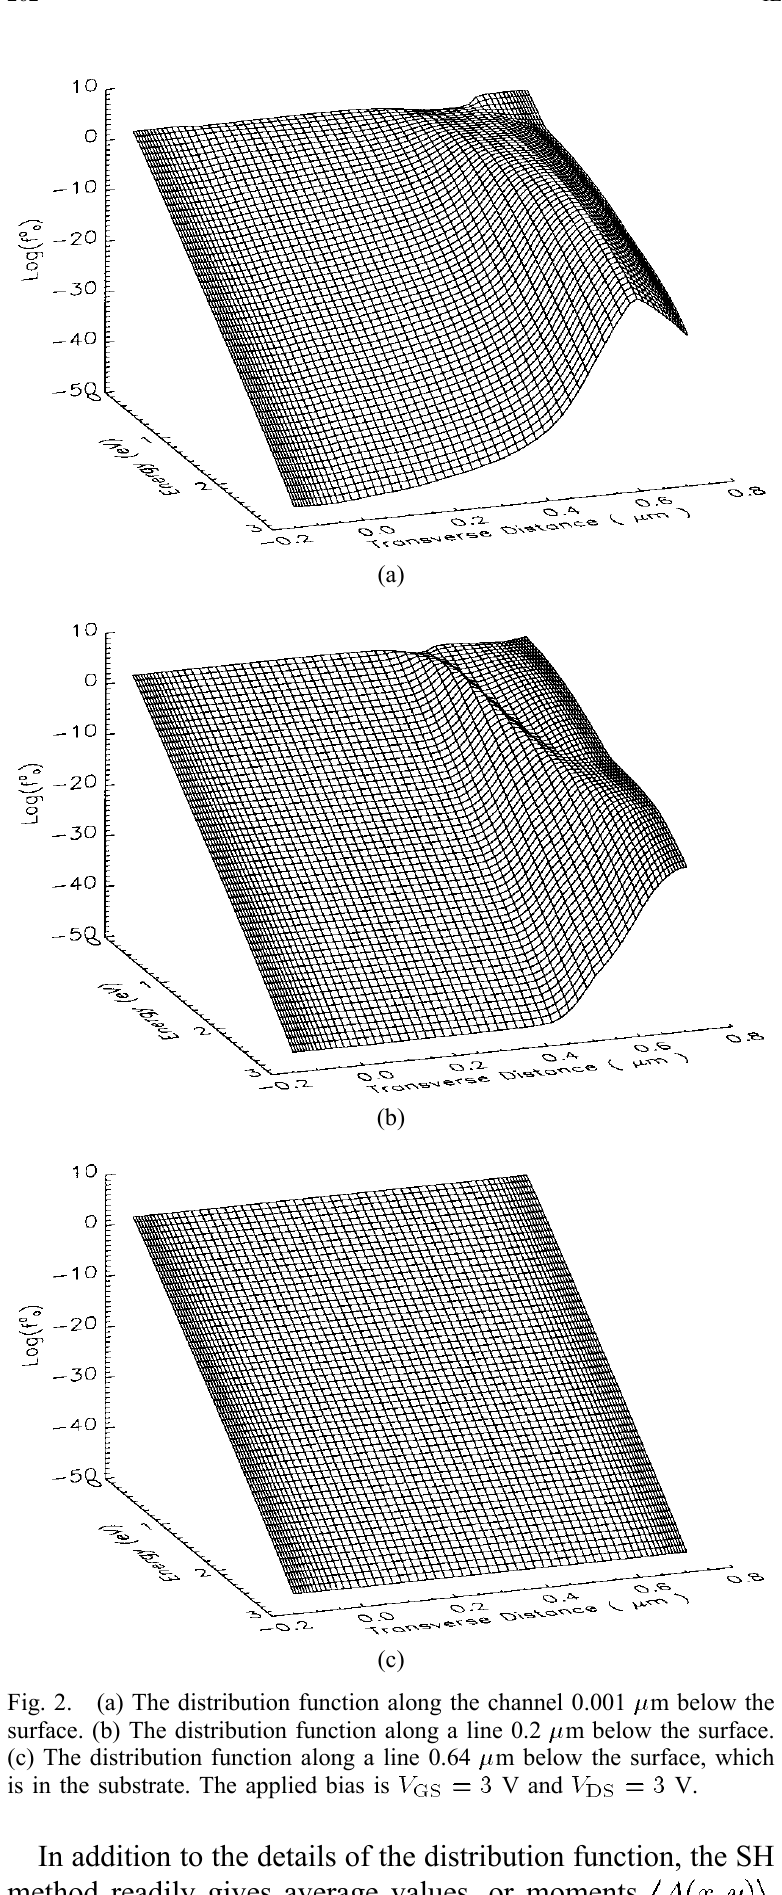
\includegraphics[height=0.44\textheight]{../figures/paper_fig2.png}\\[4pt]
{\footnotesize Liang \emph{et al.} (1997): (a) $\SI{0.001}{\micro m}$, (b) $\SI{0.2}{\micro m}$,
(c) $\SI{0.64}{\micro m}$ below the surface.}\\[10pt]
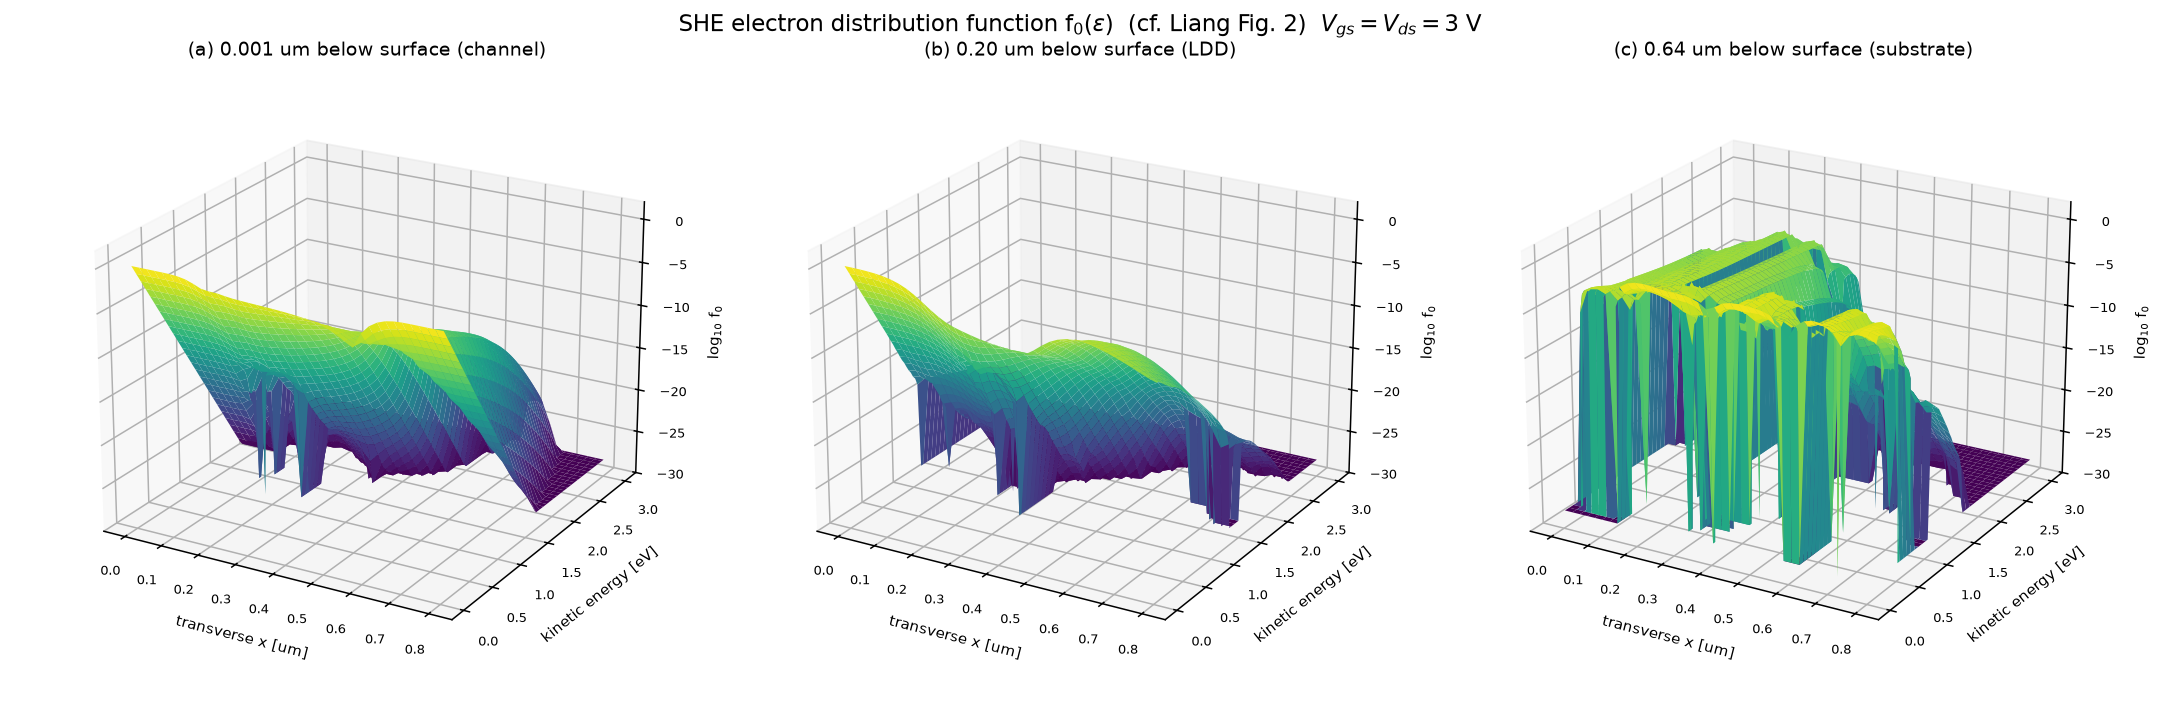
\includegraphics[width=\linewidth]{../figures/she2d_fig2_distribution.png}\\[2pt]
{\footnotesize This work (same three depths).}
\end{center}
\textbf{Comparison.} Near the surface (a) and in the LDD region (b) the distribution develops a
hot, non-Maxwellian high-energy tail toward the drain; deep in the substrate (c) it is thermal.
Our substrate slice (c) is noisier because $f_0$ there sits near the numerical floor, but the
Maxwellian plane is recovered under the noise.
\par\bigskip

\clearpage
\subsection*{Fig.~8 --- Terminal I--V characteristics}
\begin{center}
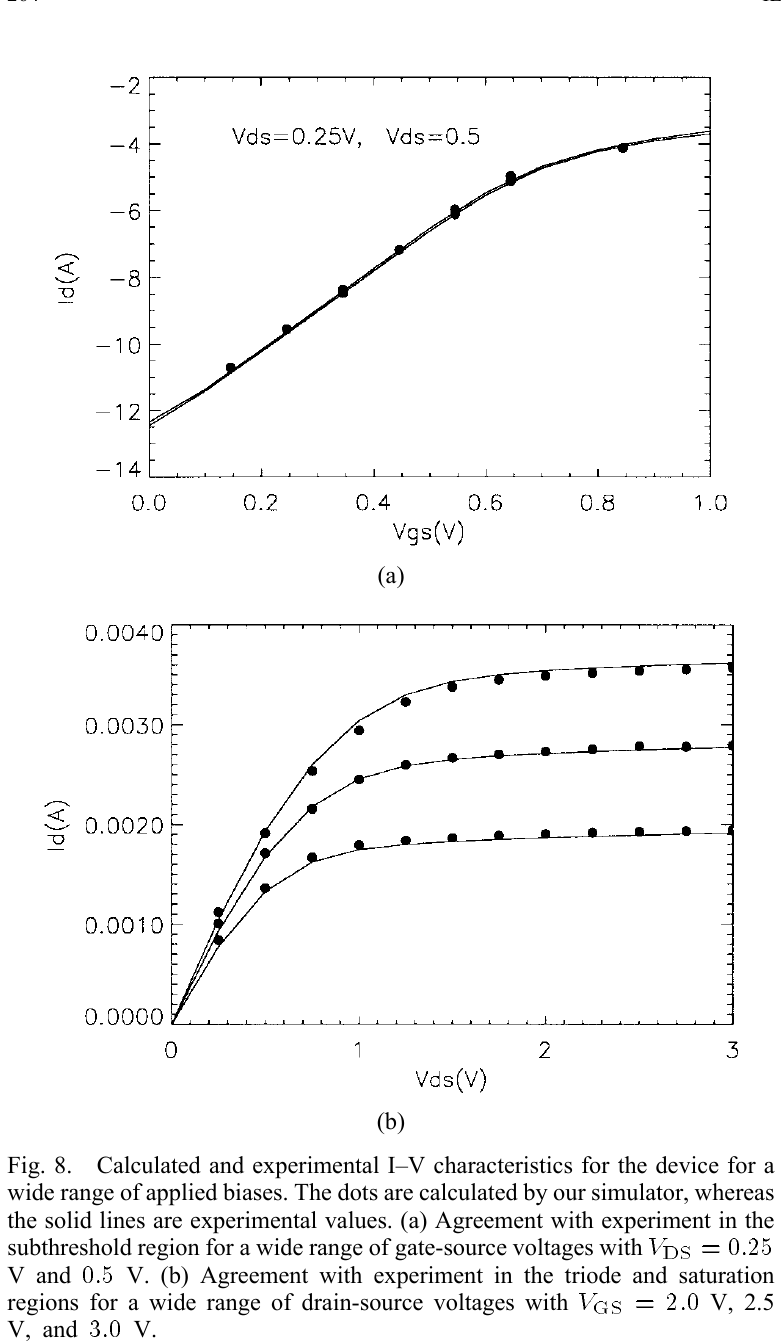
\includegraphics[height=0.44\textheight]{../figures/paper_fig8.png}\\[4pt]
{\footnotesize Liang \emph{et al.} (1997): dots = simulator, solid lines = experiment.}\\[10pt]
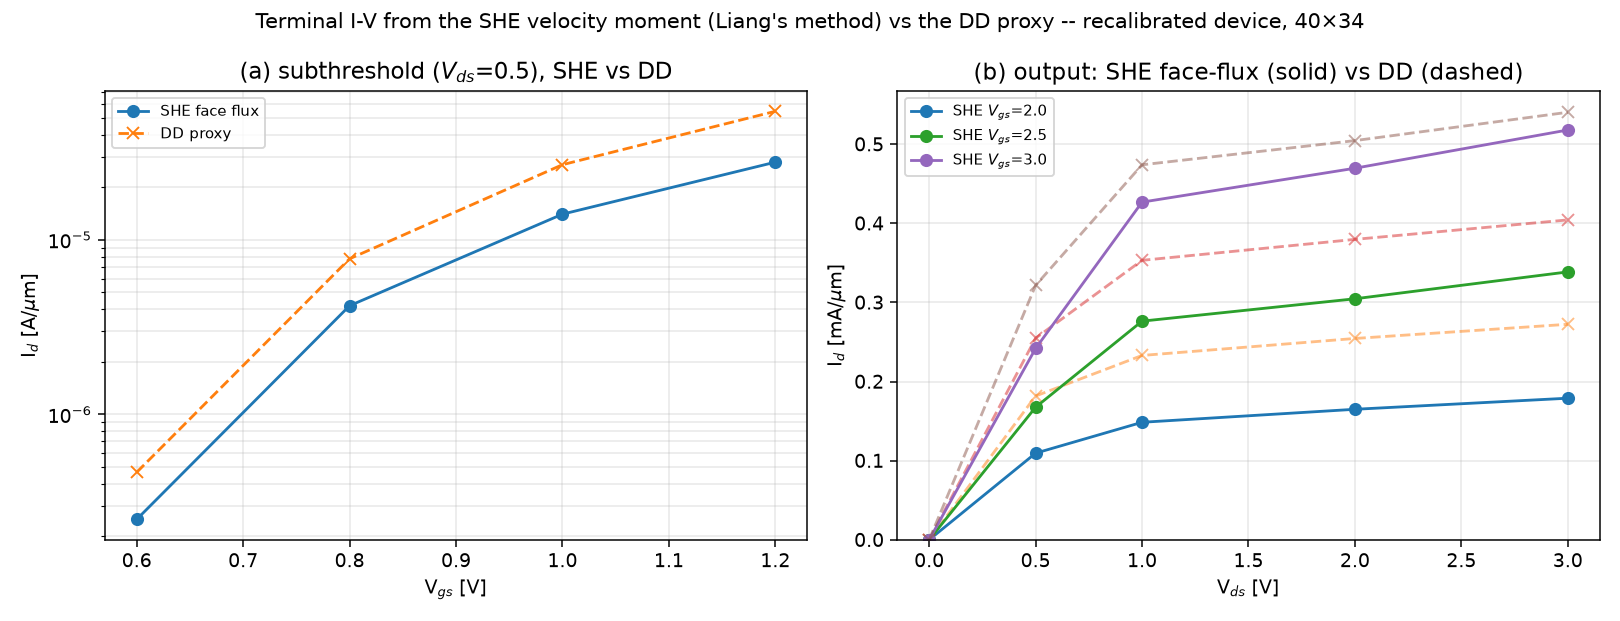
\includegraphics[width=\linewidth]{../figures/she2d_iv_moment.png}\\[2pt]
{\footnotesize This work: terminal current from the \emph{SHE velocity moment} (finite-volume face
flux, solid) vs the DD proxy (dashed), per $\mu$m.}
\end{center}
\textbf{Comparison.} Like Liang, the terminal current is obtained from the SHE velocity moment (the
finite-volume face flux), \emph{not} a mobility model, reproducing the triode$\to$saturation output
family and the monotonic $V_{gs}$ ordering; source/drain current conservation is
$2\times10^{-5}$--$10^{-3}$. The SHE current runs $I_{d,\text{SHE}}/I_{d,\text{DD}}=0.51$--$0.96$
(bias-dependent), systematically below the DD proxy retained (dashed) for comparison. This is a
\emph{one-way} SHE (on the DD potential), and the subthreshold panel is at $V_{ds}=\SI{0.5}{V}$ only
--- a partial reproduction of Liang's 0.25/0.5-V Fig.~8(a) family. Liang's Fig.~8 solid lines are
moreover experimental data for a real device of unstated width, so only the per-width \emph{shape}
is comparable, not the absolute ampere magnitude.

\end{document}
